\begin{frame}
	\frametitle{Robots de ficción}
	\begin{figure}[!h]
		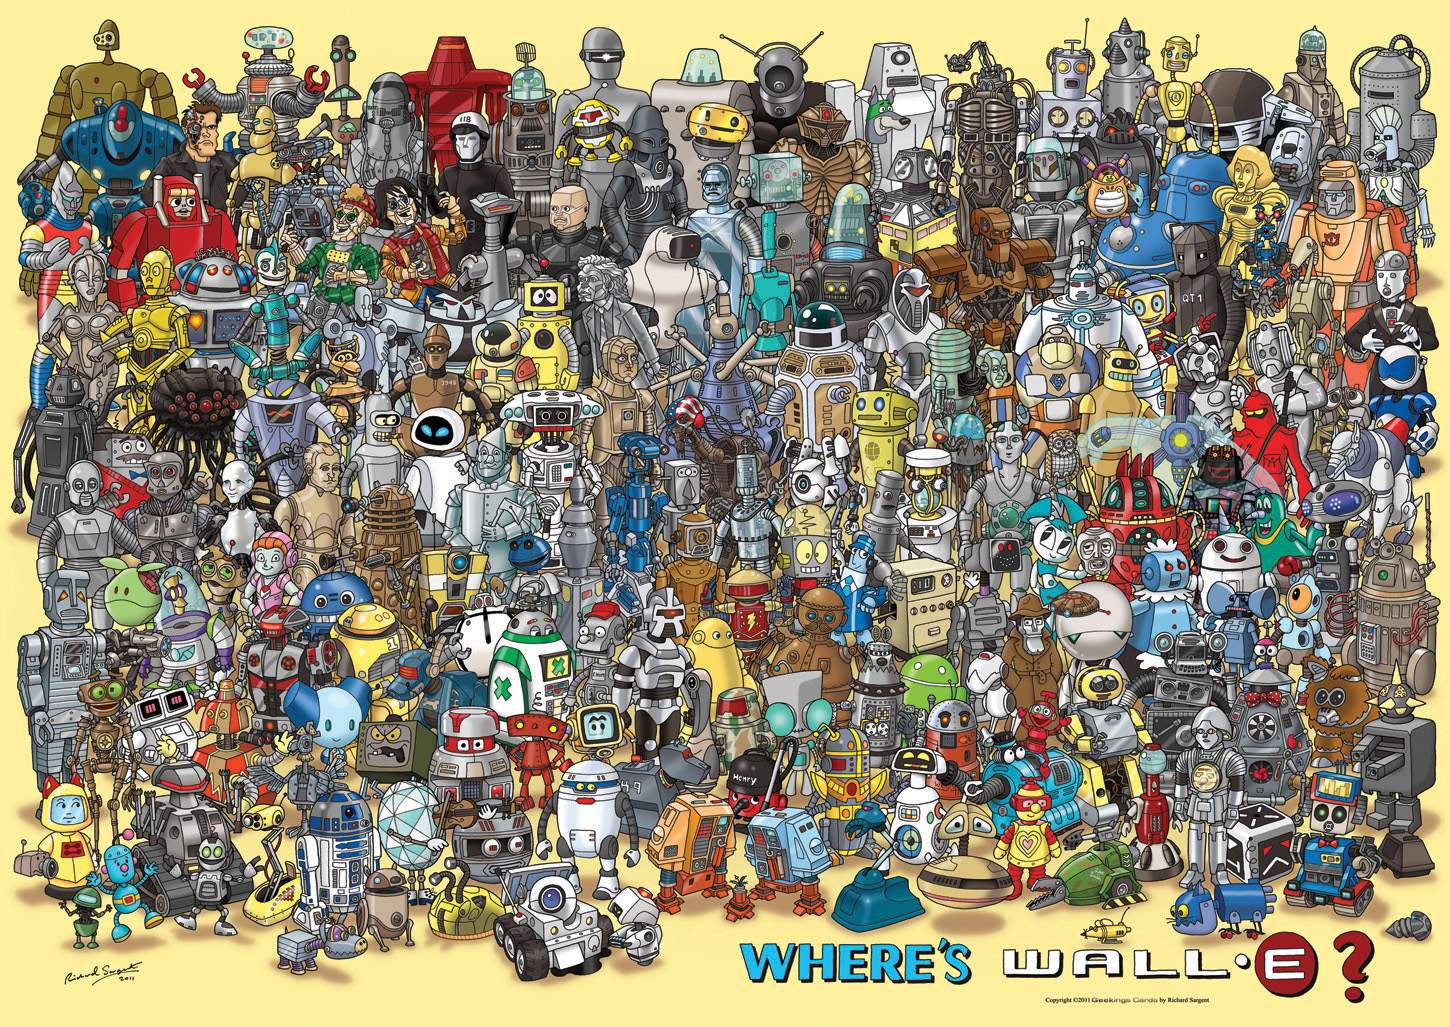
\includegraphics[width=0.7\columnwidth]{wheres_wall_e_poster.jpg}
     \end{figure}
\end{frame}

\begin{frame}
	\frametitle{Robots de ficción}
	
	\begin{figure}
		\centering
		\subfloat[]
		{
			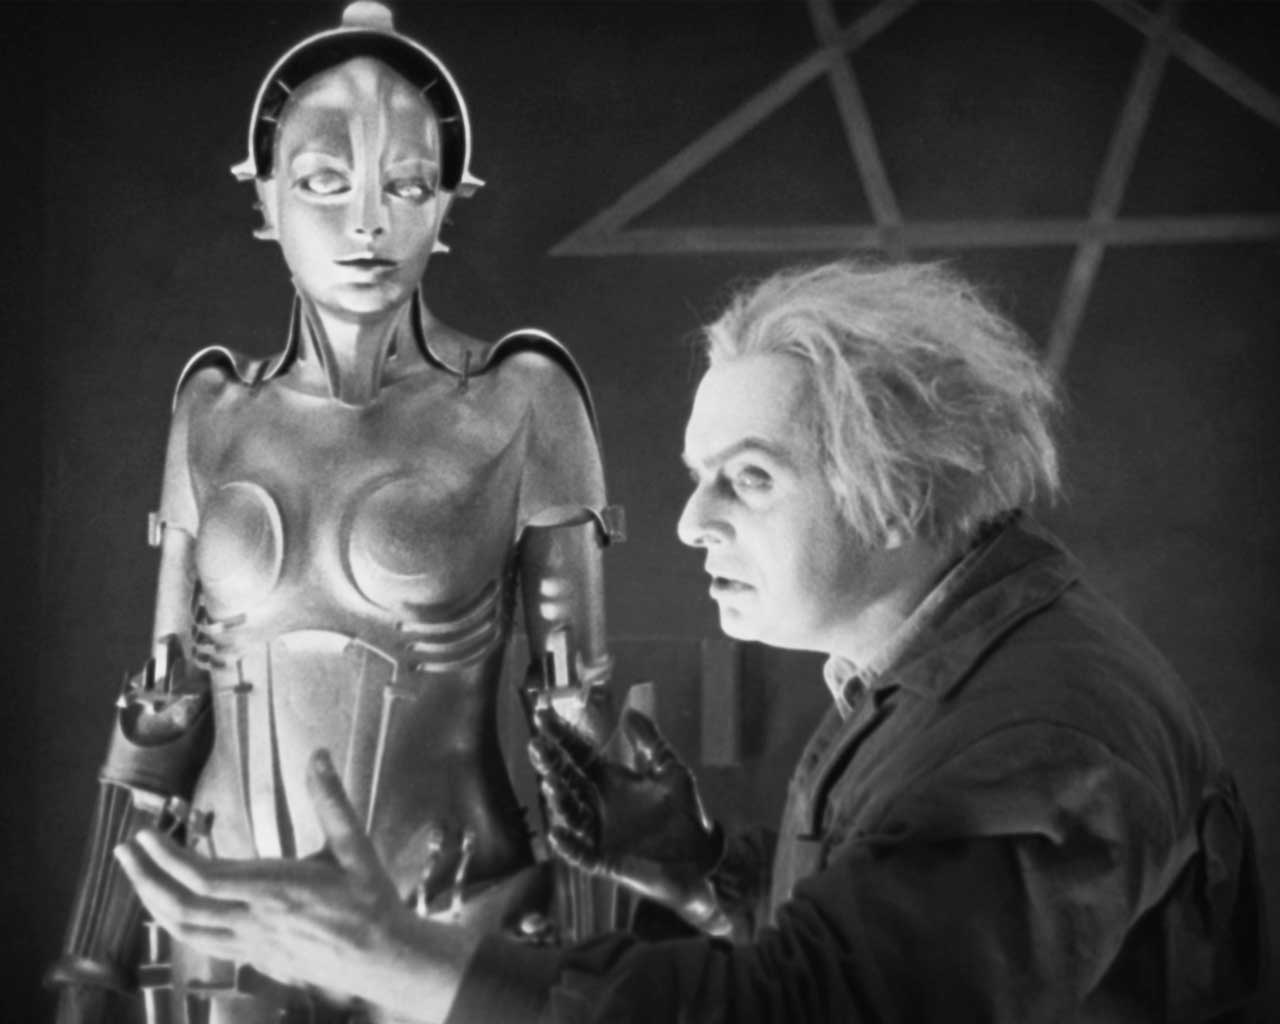
\includegraphics[width=0.3\columnwidth]{images/maria_movie_metropolis_1927.jpg}
		}
		\subfloat[]
		{
			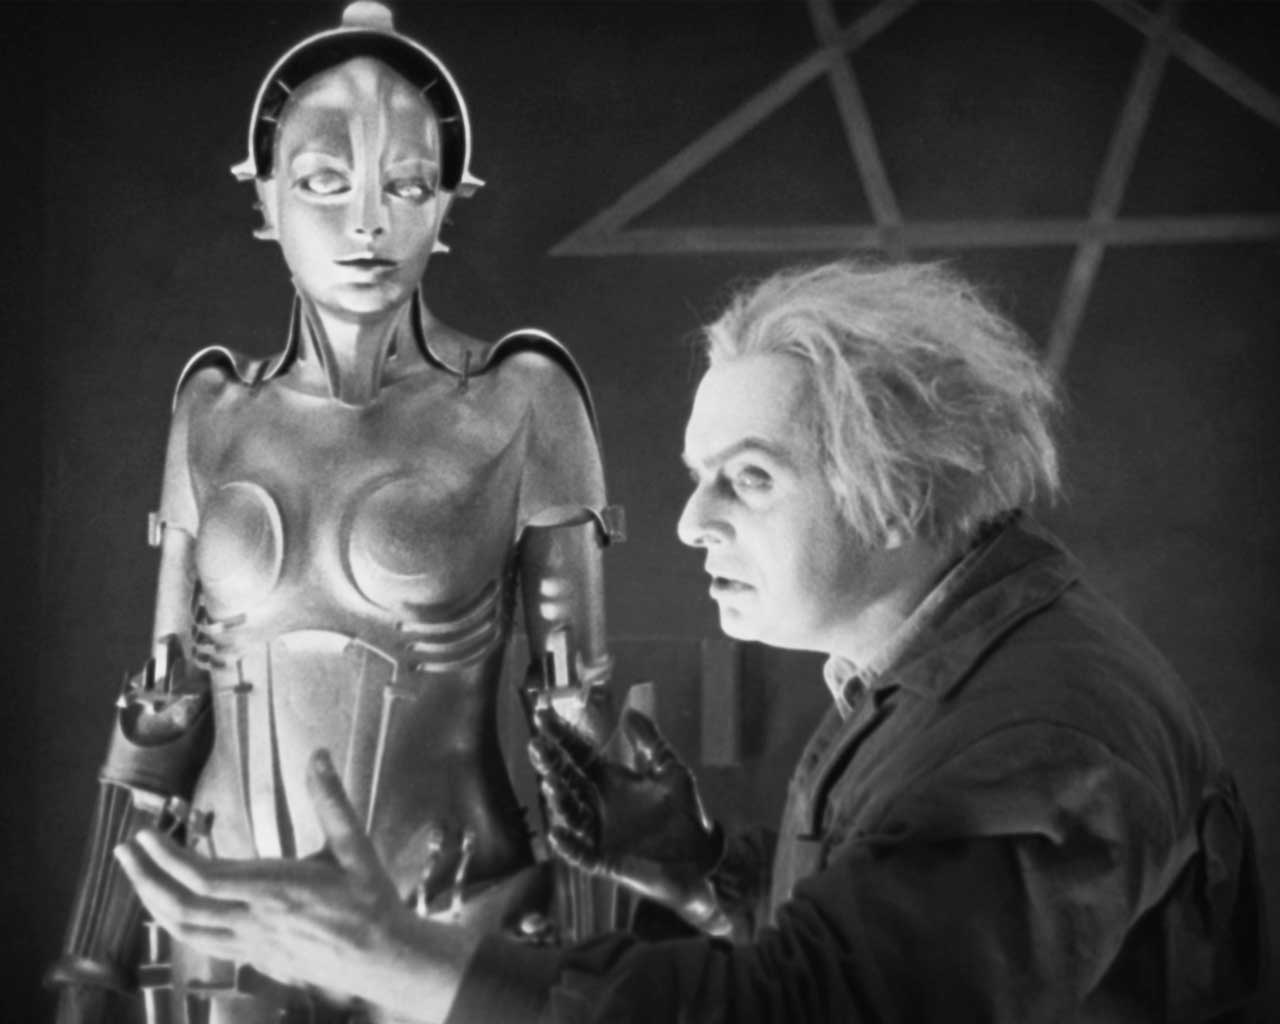
\includegraphics[width=0.4\columnwidth]{images/maria_movie_metropolis_1927.jpg}
		}
	\end{figure}
	
	\TODO{Agregar slides de robots de ficción. como Hace peter corke: https://robotacademy.net.au/masterclass/introduction-to-robotics/?lesson=211}
\end{frame}

\begin{frame}
	\frametitle{¿Qué es un Robot?}
	
	\begin{block}{Según Robot Institute of America, 1979}
		Un manipulador reprogramable y multifuncional diseñado para mover material, piezas, herramientas o dispositivos especializados a través de varios movimientos programados para el desempeño de una variedad de tareas.
	\end{block}
	
	\begin{block}{Según la RAE}
		Máquina o ingenio electrónico programable que es capaz de manipular objetos y realizar diversas operaciones.
	\end{block}
	
	\begin{block}{Una definición que usamos (\url{https://robots.ieee.org/learn/what-is-a-robot/}):}
		Un robot es una máquina autónoma capaz de sensar su entorno, realizar cálculos para tomar decisiones y realizar acciones en el mundo real.
	\end{block}
	
	\note{hay varias definiciones.\\
		Fuente: https://robots.ieee.org/learn/what-is-a-robot/}
\end{frame}

\begin{frame}
	\frametitle{¿Qué es la Robótica?}
	
	\begin{block}{Robótica}
	La Robótica es la intersección de la ciencia, la ingeniería y la tecnología que produce máquinas, llamadas robots, que sustituyen (o replican) las acciones humanas.
	\end{block}
	
	\begin{block}{Mecatrónica}
	La Mecatrónica tiene como objetivo el diseño y desarrollo de sistemas inteligentes y automatizados que puedan interactuar con el entorno y adaptarse a diferentes situaciones. Los sistemas mecatrónicos pueden incluir robots, pero también abarcan una amplia gama de productos y sistemas que no necesariamente son robots (como electrodomésticos, dispositivos médicos, etc).
	\end{block}
	
	\begin{block}{La Domótica}
	La domótica se refiere a la automatización y control inteligente de los sistemas y aparatos del hogar para mejorar la calidad de vida, la eficiencia energética y la seguridad. La palabra ``domótica'' proviene de la unión de las palabras ``domus'' (hogar en latín) y ``robótica''.
	\end{block}
	
\end{frame}


\begin{frame}
    \frametitle{Un poco de Historia}

    La primera aparición de la palabra robot es utilizada por Karl Capek en 1921 en su obra teatral R. U. R. (Rossumovi Univerzální Roboti Rossum's Universal Robots). La palabra robot viene de la palabra checa \emph{robota} que significa esclavo.


    \centering
    \begin{figure}
    	\subfloat[]
    	{
    		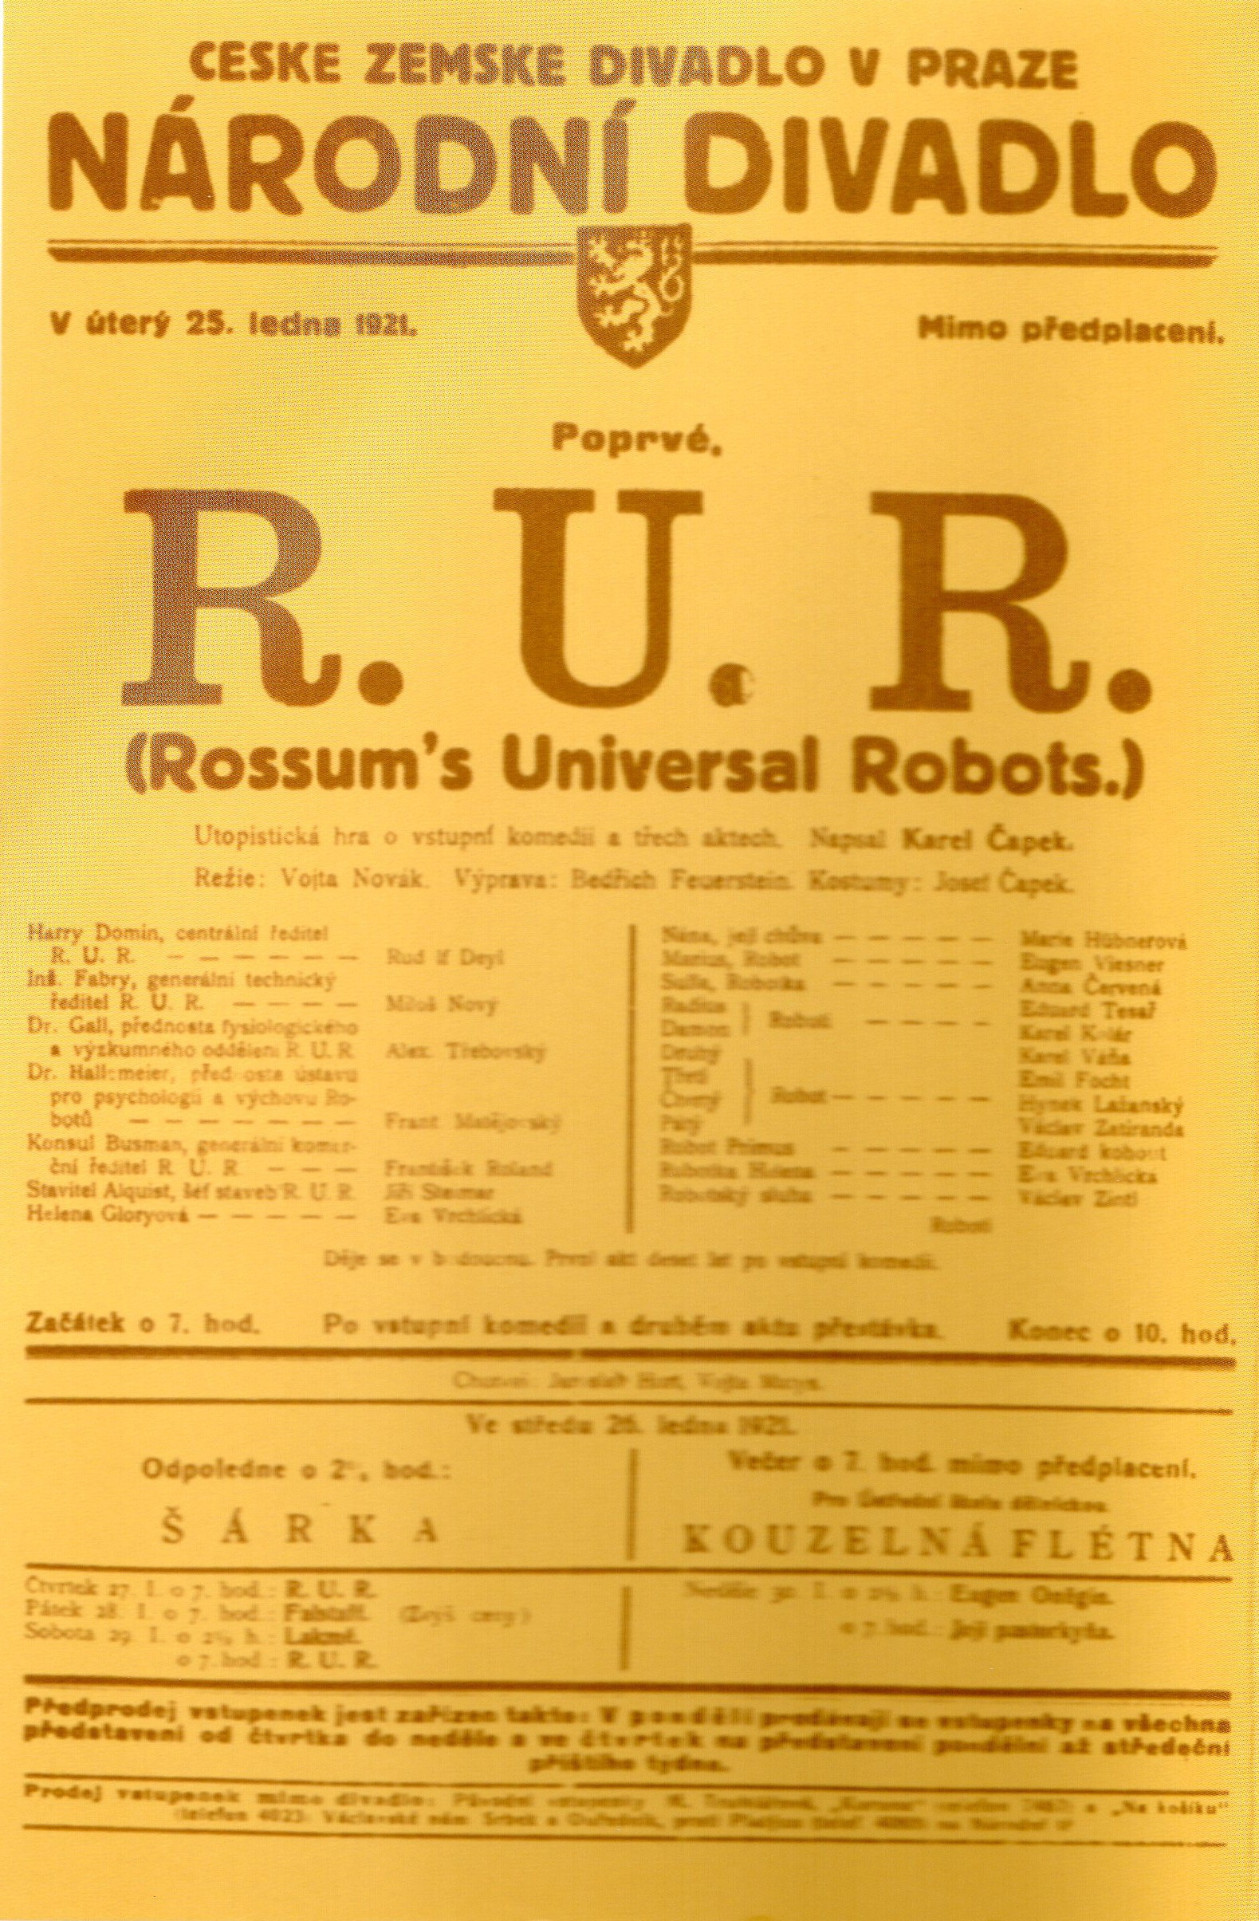
\includegraphics[width=0.2\columnwidth]{rossums_universal_robots_poster.jpg}
    	}\hfill
    	\subfloat[]
    	{
   			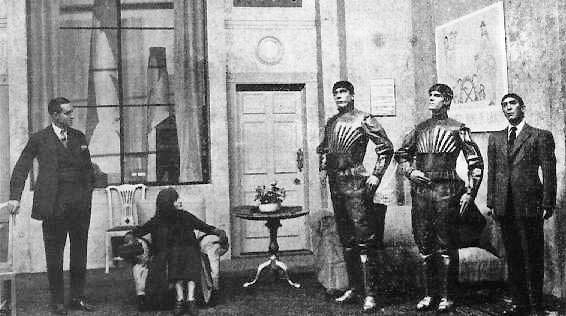
\includegraphics[width=0.5\columnwidth]{rossums_universal_robots_play.jpg}
    	}
    \end{figure}

    \note{
        Fuente: https://cs.stanford.edu/people/eroberts/courses/soco/projects/1998-99/robotics/history.html\\
        La obra teatral trata sobre una empresa que construye humanos artificiales orgánicos con el fin de aligerar la carga de trabajo del resto de personas. Aunque en la obra a estos hombres artificiales se les llama robots, tienen más que ver con el concepto moderno de androide o clon. Se trata de criaturas que pueden hacerse pasar por humanos y que tienen el don de poder pensar. Pese a ser creadas para ayudar a la humanidad, más adelante estas máquinas entrarán en confrontación con la sociedad, iniciando una revolución que acabará destruyendo la humanidad.}
\end{frame}

\begin{frame}
    \frametitle{Un poco de Historia}

    La palabra \emph{robotics} también fue utilizada por primera vez por Issac Asimov en 1942 en su cuento corto \emph{Runaround} (en español Circuito Vicioso).

    \begin{itemize}
        \item Primera Ley: Un robot no hará daño a un ser humano ni, por inacción, permitirá que un ser humano sufra daño.
        \item Segunda Ley: Un robot debe cumplir las órdenes dadas por los seres humanos, a excepción de aquellas que entren en conflicto con la primera ley.
        \item Tercera Ley: Un robot debe proteger su propia existencia en la medida en que esta protección no entre en conflicto con la primera o con la segunda ley.
    \end{itemize}


    \note{The word robotics was also coined by a writer.  Russian-born American science-fiction writer Isaac Asimov first used the word in 1942 in his short story Runabout.  Asimov had a much brighter and more optimistic opinion of the robot's role in human society than did Capek.  He generally characterized the robots in his short stories as helpful servants of man and viewed robots as a better, cleaner race.  Asimov also proposed three "Laws of Robotics" that his robots, as well as sci-fi robotic characters of many other stories.}
\end{frame}

\begin{frame}
	\frametitle{Autómata 1808-1840}
	\note{Agregar un timeline de robotica: https://robotacademy.net.au/masterclass/introduction-to-robotics/?lesson=215}
	
	\note{1808-1840 Autómata. Maquínas que funcionaban como un reloj.}
	
	\begin{figure}
		\centering
		\subfloat[]
		{
			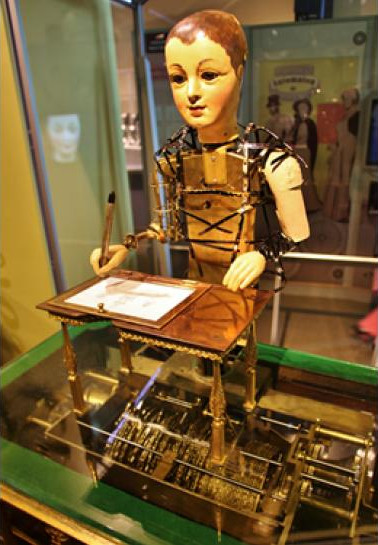
\includegraphics[width=0.3\columnwidth]{images/maillardet_automata_1808.jpg}
		}
		\subfloat[]
		{
			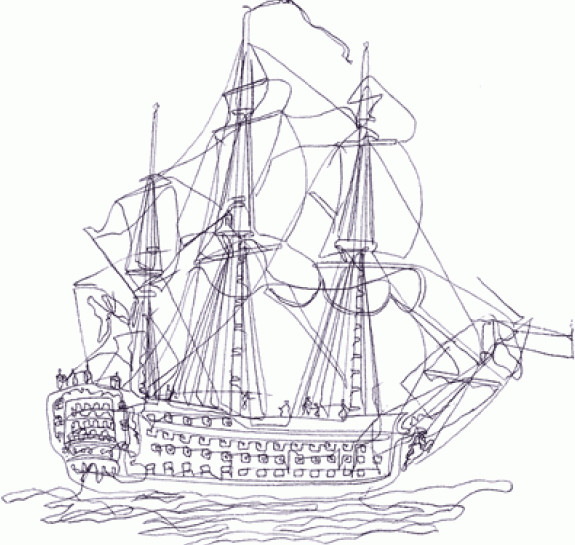
\includegraphics[width=0.4\columnwidth]{images/maillardet_automata_draw_1808.jpg}
		}
	\end{figure}
	
\end{frame}

\begin{frame}
	\frametitle{Telar de Jacquard 1801}
	
	\note{https://robotacademy.net.au/masterclass/introduction-to-robotics/?lesson=215}
	
	\begin{figure}[!h]
		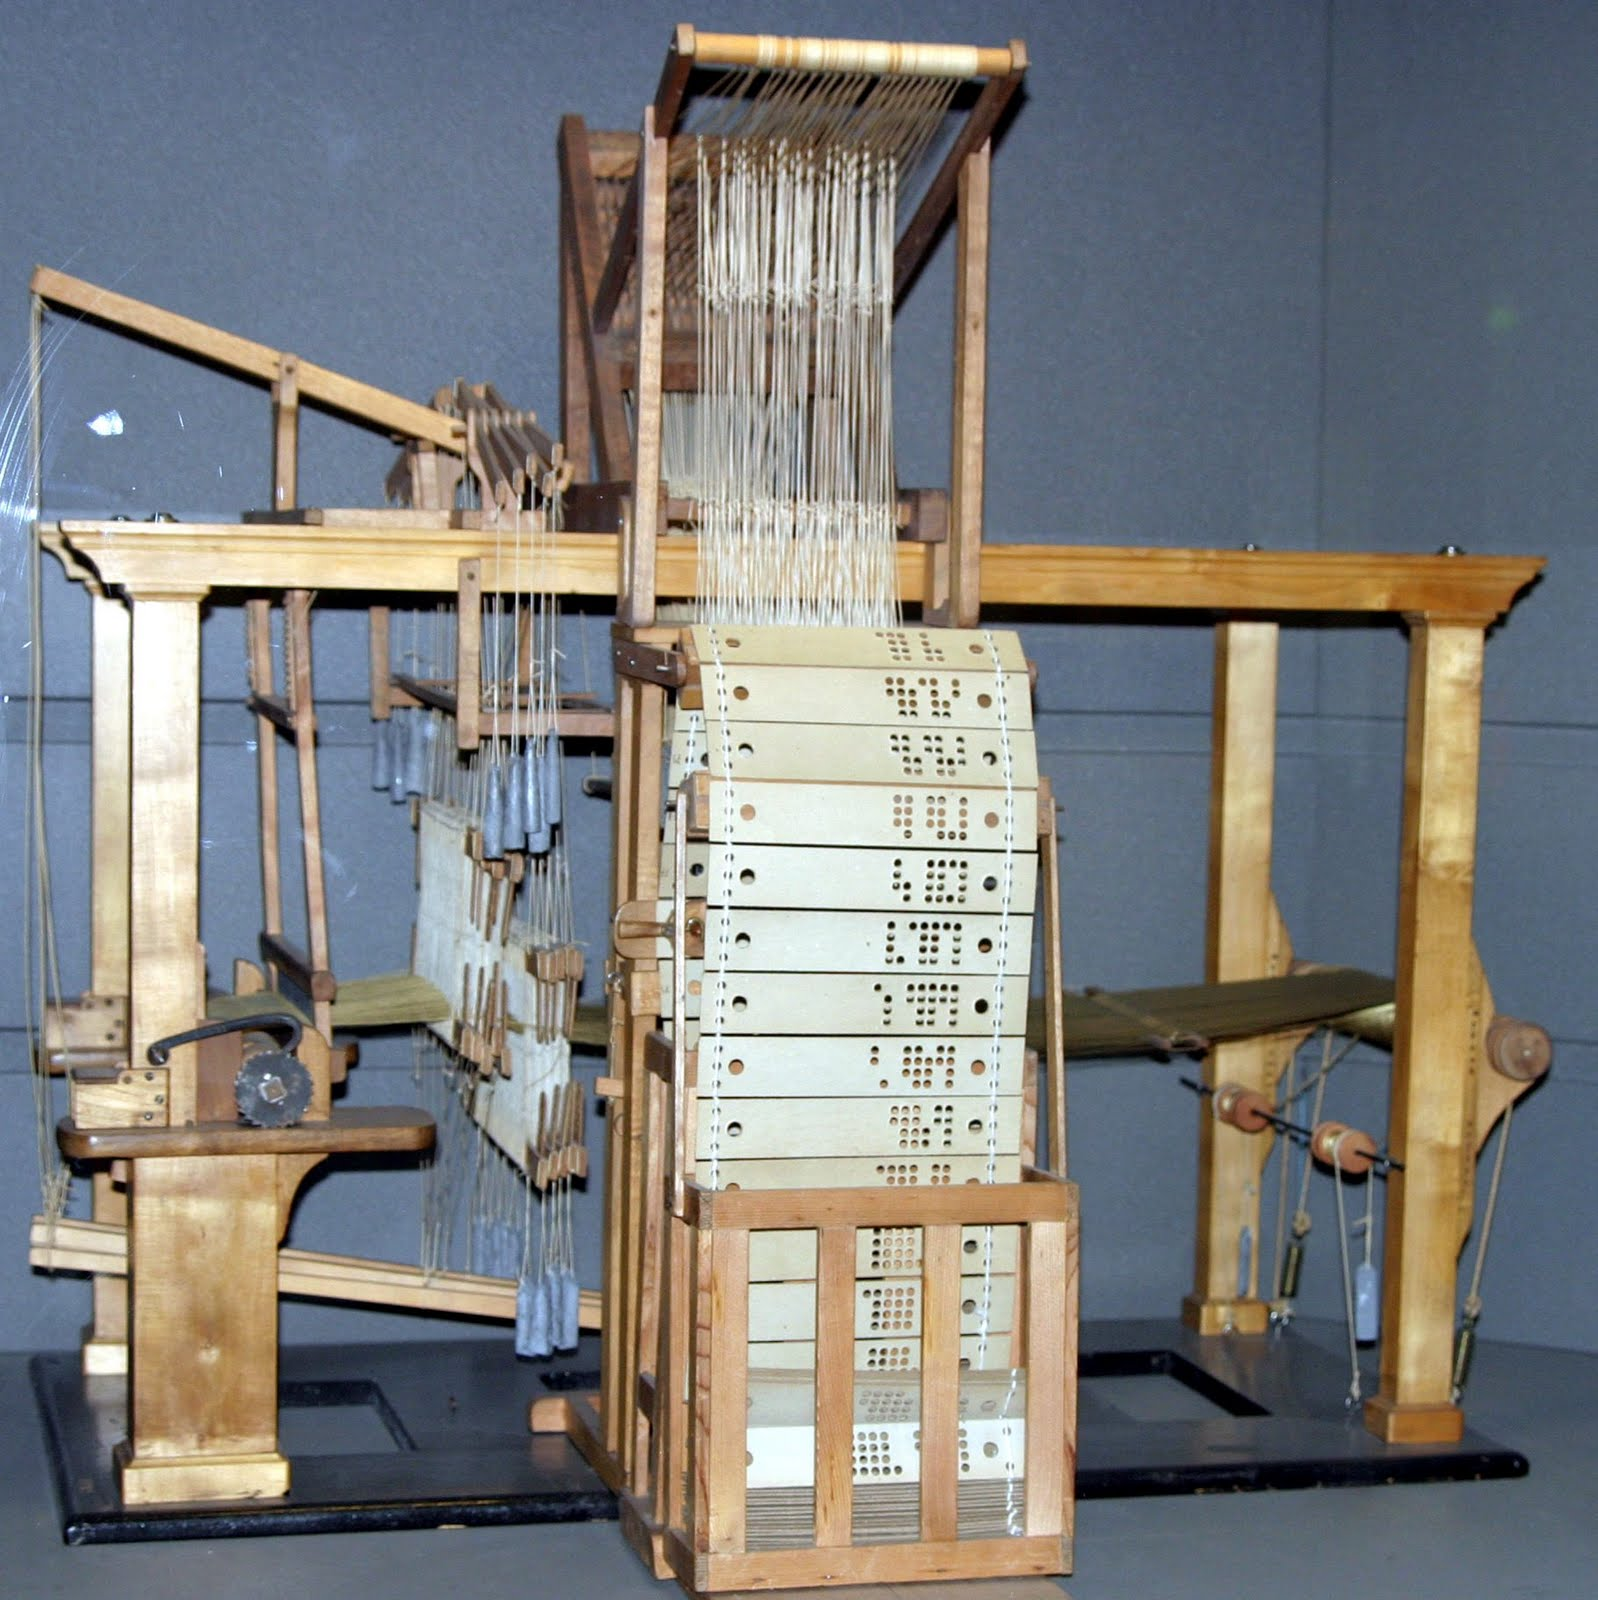
\includegraphics[width=0.5\columnwidth]{images/jacquard_loom_1801.jpg}
	\end{figure}
	
	\note{El artilugio utilizaba tarjetas perforadas para conseguir tejer patrones en la tela, permitiendo que hasta los usuarios más inexpertos pudieran elaborar complejos diseños.
		
	Aunque siempre se ha denominado telar de Jacquard, el telar de Jacquard en sí es la máquina inferior que intersecciona los hilos para producir la tela, mientras que lo que verdaderamente inventó Jacquard es la máquina que produce el movimiento independiente de los hilos de urdimbre para conseguir el dibujo solicitado a través de las armuras o ligamentos insertados en las diferentes zonas del tejido.
	
	Cada tarjeta perforada correspondía a una línea del diseño, y su colocación junto con otras tarjetas determinaba el patrón (ligamento/armura) con el que el telar tejería. Cada agujero de la tarjeta correspondía con un gancho "Bolus", que tenía dos posiciones, pudiendo estar arriba o abajo. De esta manera, dependiendo de qué posición tuviera, el arnés (montura) que lleva y guía la urdimbre haría que la trama se desplazara hacia arriba o hacia abajo. De esta manera, la secuencia de subidas y bajadas del hilo termina por crear un patrón (ligamento/armura) sobre el tejido. Los ganchos o pestañas podían ser conectados a través del arnés con un determinado número de hilos, permitiendo que el patrón (camino) se repitiera más de una vez.
	
	Un telar con 400 ganchos podía tener conectados hasta cuatro hilos por gancho, produciendo así una tela con una anchura de 1600 hilos, y con un patrón compuesto por la combinación de las repeticiones de cuatro bandas.}
	
\end{frame}

\begin{frame}
	\frametitle{Máquina diferencial de Babbage 1870}
	
	\note{https://robotacademy.net.au/masterclass/introduction-to-robotics/?lesson=215}
	
	Una máquina diferencial es una calculadora mecánica de propósito especial, diseñada para calcular funciones polinómicas. La Máquina diferencial mecánica creada por Babbage utiliza tarjetas perforadas para realizar cómputos. Aunque no fue construida en su momento fijo los cimientos para construir la computadora electrónica ENIAC durante la Segunda Guerra Mundial.
	
	\begin{figure}[!h]
		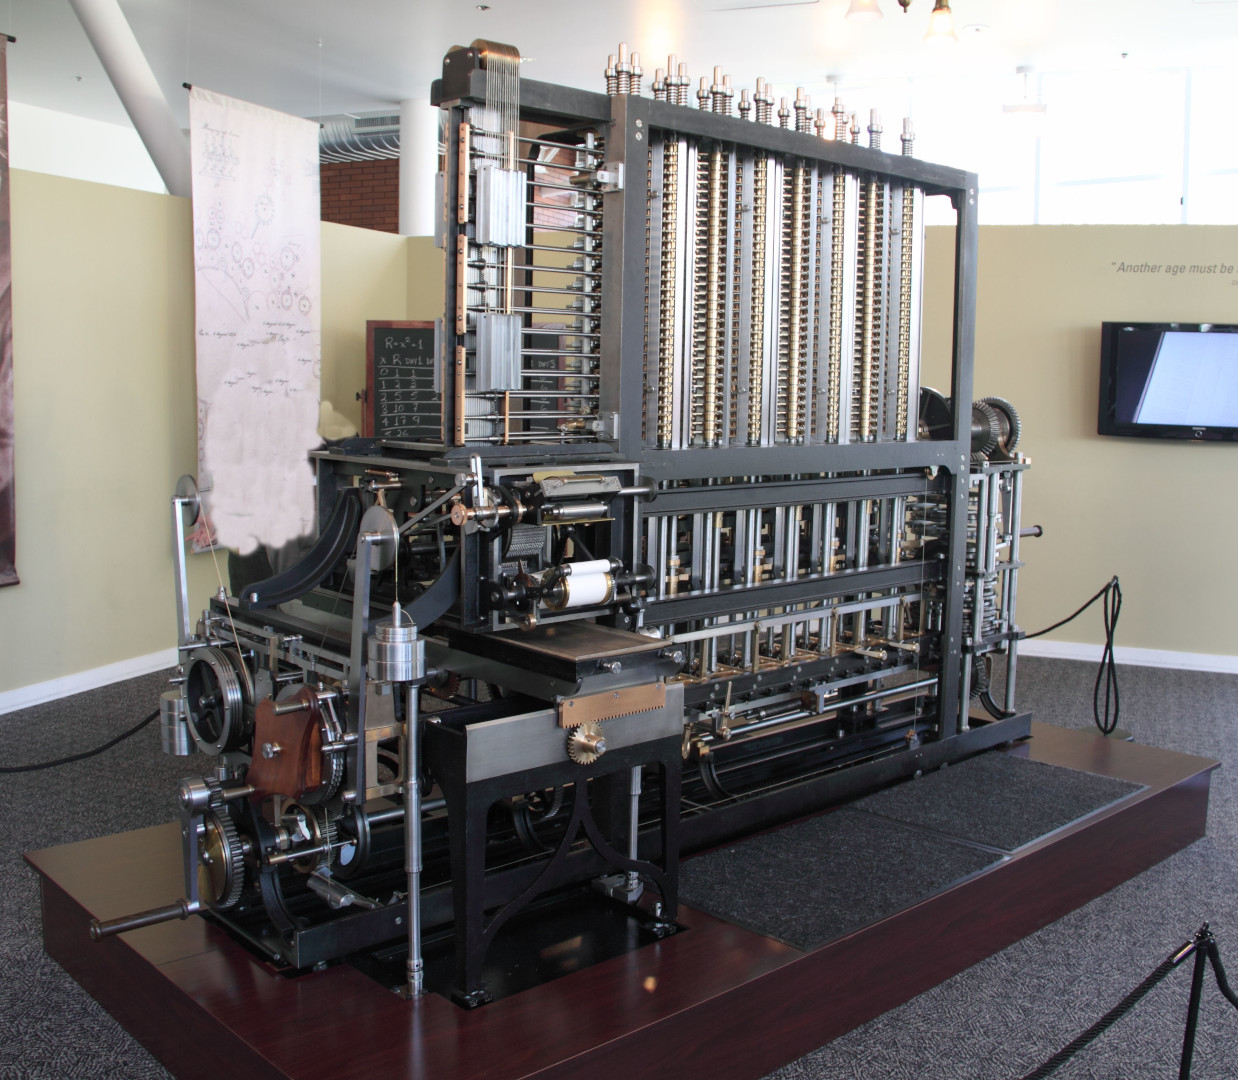
\includegraphics[width=0.5\columnwidth]{images/babbage_difference_engine_1870.jpg}
	\end{figure}

	\note{The notion of punch card control was picked up by Charles Babbage, when he was conceiving a mechanical computing engine in the late 1800s. At that time he didn't have the technology to actually build this machine but he introduced the really important notion of a general-purpose computing engine and the computation that it performed is dictated by a program. In his case, input on punched cards.
	
	The ideas embodied in this machine influenced later electronic computing devices. For an instance, the ENIAC Computer that was built during World War II and from that machine, we can trace a lineage to the computers we use every day, in our laptops and in our mobile phones, and computers of course, are a critical component of robot systems that we build today. We can perhaps think of a robot as a computer that can do things to the physical world.}
	
\end{frame}


\begin{frame}
	\frametitle{Teleoperación por Raymond Goertz 1949}

	\note{https://robotacademy.net.au/masterclass/introduction-to-robotics/?lesson=215}
	Máquinas maestro-esclavo para manipular materiales radioactivos durante la construcción de armas nucleares. Nace la teleoperación.
	\begin{figure}[!h]
	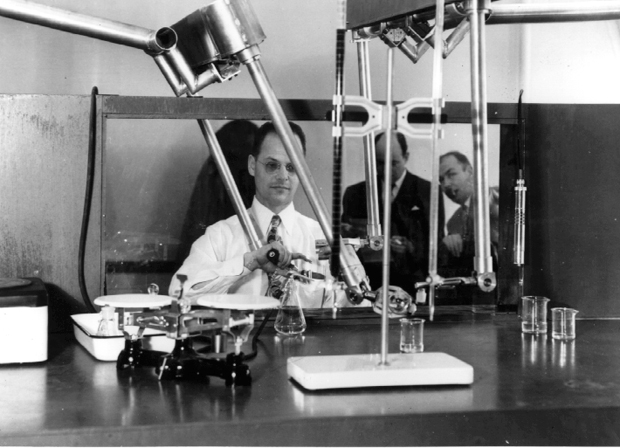
\includegraphics[width=0.6\columnwidth]{images/raymond_goertz_1949.jpg}
	\end{figure}

	\note{The other really important innovation that led to robotics as we know them today is this work that was done after World War II at the Argonne National Laboratory in the United States. In there, they were faced by a problem of assembling nuclear weapons. This required them to handle, to manipulate pieces of material that were radioactive. This was a task that couldn't be undertaken by human beings because it would injure or kill the people who did that work. We needed to have machines to handle that material instead but the problem was that we need a lot of skill and intelligence in order to manipulate this radioactive material, so, they came up with a concept called teleoperation.
		
	The people in white coats are sitting with what are called the master manipulator arms so they would grab those arms with their hands and they would move them. The arms over here are referred to as the slave arms. They move in such a way as to mimic the motion of the master arm. So, the people who were doing the assembly work and controlling the master arms, the slave arms are in a remote room performing work on the radioactive material. Video of what’s going on in the radioactive room is transmitted back to the people doing the work with the master arm so they can see what’s happening on a TV monitor. They move the master arms, the slave arms move in synchronism and perform the task remotely. This is a technique called teleoperation. It’s not really robotic. In some ways, you can think of it as a very-sophisticated, remote-controlled technology. It was really important to achieve this specific task at the Argonne National Laboratory.
		
	This technology is an important precursor to modern manufacturing robots. What we do is we cut the wire between the master arm and the slave arm and instead of the master arm sending the commands to the slave arm, we put a computer there instead. So, the computer is sending commands to the slave arm which is going to move in accordance to the signals coming out of the computer. Of course, the computer is an infinitely reprogrammable device so therefore we can make the slave arm do anything that we like at all and now, there are no longer any human beings involved. We've created a robot.}

\end{frame}

\begin{frame}
	\frametitle{Standford Cart 1961}
	
	\begin{figure}[!h]
		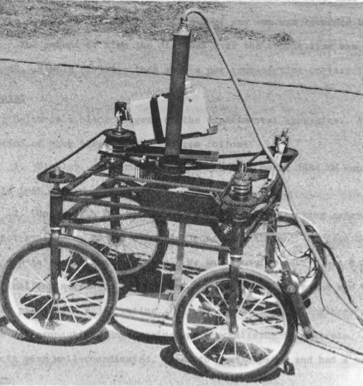
\includegraphics[width=0.4\columnwidth]{images/standford_cart_1961.png}
	\end{figure}
	
	\note{1960-61 - The Stanford Cart was originally constructed by Mechanical Engineering (ME) graduate student James L. Adams to support his research on the problem of controlling a remote vehicle using video information. He had been working at the Jet Propulsion Laboratory on a NASA project called Project Prospector, which was proceeding with the assumption that someone on earth could drive around the Moon using a TV camera on a vehicle and a radio control link However Adams showed that assumption to be false.
		
	The Cart had four small bicycle wheels with electric motors powered by a car battery and carried a television camera with a fixed view in the forward direction. Tests were conducted using both 2-wheel steering, like a car, and 4-wheel steering, in which the wheels and television camera swivel together. The cart was connected by a very long cable to a control console with a television display and controls for steering and speed. A magnetic tape loop made it possible to vary the time delay of steering commands, to simulate communication delays.
	
	Adams explored the controllability of the vehicle while avoiding obstacles with various combinations of communication delay and speed. When steering commands are delayed by communications there is a tendency for the operator to over-steer and lose control. Among other things, Adams showed in his dissertation that with a communication delay corresponding to the round trip to the Moon (about 2 1/2 seconds) the vehicle could not be reliably controlled if traveling faster than about 0.2 mph (0.3 kph).}
\end{frame}

\begin{frame}
	\frametitle{Unimation Inc 1956}
	
	\begin{figure}[!h]
		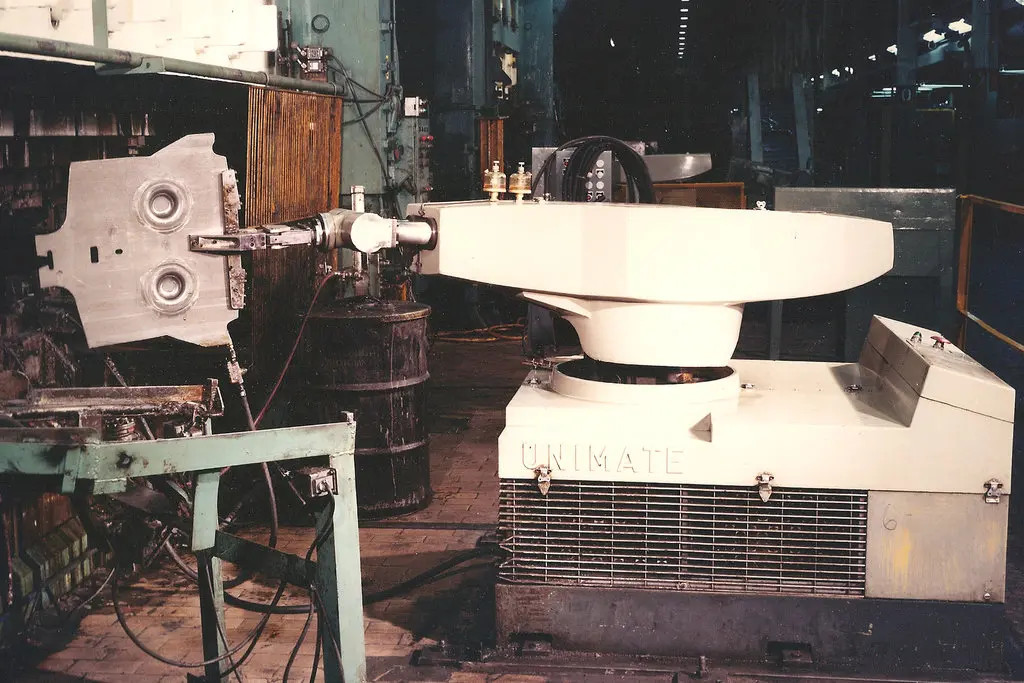
\includegraphics[width=0.7\columnwidth]{images/devol_robot_arm_1956.jpg}
	\end{figure}

	\note{This technology is an important precursor to modern manufacturing robots. What we do is we cut the wire between the master arm and the slave arm and instead of the master arm sending the commands to the slave arm, we put a computer there instead. So, the computer is sending commands to the slave arm which is going to move in accordance to the signals coming out of the computer. Of course, the computer is an infinitely reprogrammable device so therefore we can make the slave arm do anything that we like at all and now, there are no longer any human beings involved. We've created a robot.
		
	And perhaps the person that this idea first occurred to is George Devol, gentleman shown here, prolific American inventor who died only recently. He had the idea of creating what he called universal automation which was contracted to Unimation. That was the name of the company that he founded in 1956 with Joseph Engelberger. They founded the company to produce industrial robots that would eventually go to work in general motors plants. The first of their robots which was installed in 1961 is shown here. What this robot did was to unload castings from a die-casting machine.
	
	This was the start of the revolution of robots working in the manufacturing industry. Unimation, Inc. was the first company to build manufacturing robots. They were the pioneers. They’re no longer in business and today, there are many, many companies that build manufacturing robots, but most of them can trace their ancestry, their ideas or perhaps even the people back to this little company founded in 1956 in Connecticut in the United States.}

\end{frame}

\begin{frame}
    \frametitle{Shakey the robot: el primer robot móvil autónomo}


    \begin{columns}[T] % align columns
        \begin{column}{.4\textwidth}
            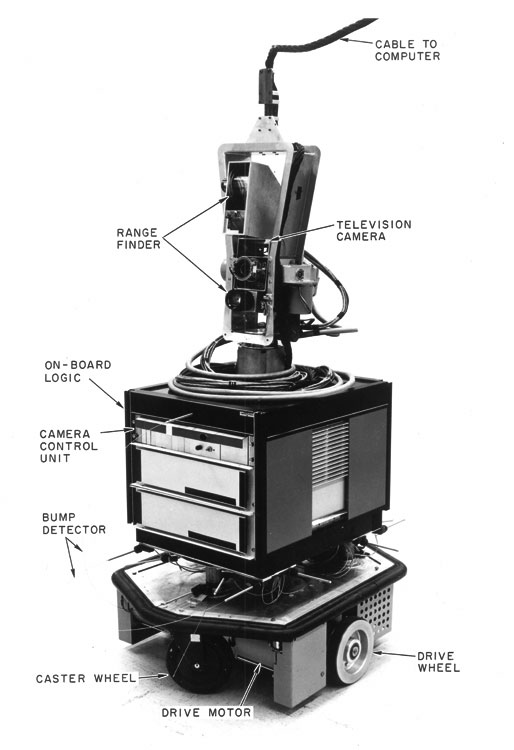
\includegraphics[width=0.8\columnwidth]{shakey.png}
        \end{column}%
        \hfill%
        \begin{column}{.56\textwidth}
              Desarrollado durante 1966 - 1972 por Stanford Research Institute International (SRI).

              Resultados: A*, Hough transform y visibility graph.

        \end{column}%
    \end{columns}

    \note{Fueten: Wikipedia\\
        Shakey experienced a limited world. A version of Shakey's world could contain a number of rooms connected by corridors, with doors and light switches available for the robot to interact with.\\
        The development of Shakey had a far-reaching impact on the fields of robotics and artificial intelligence, as well as computer science in general. Some of the more notable results include the development of the A* search algorithm, which is widely used in pathfinding and graph traversal, the process of plotting an efficiently traversable path between points; the Hough transform, which is a feature extraction technique used in image analysis, computer vision, and digital image processing; and the visibility graph method for finding Euclidean shortest paths among obstacles in the plane\\
        An example mission for Shakey might be something like:\\
        An operator types the command push the block off the platform at a computer console. Shakey looks around, identifies a platform with a block on it, and locates a ramp in order to reach the platform. Shakey then pushes the ramp over to the platform, rolls up the ramp onto the platform, and pushes the block off the platform. Mission accomplished.}
\end{frame}

\begin{frame}
    \frametitle{Aplicaciones de la Robótica}

    \note{https://robots.ieee.org/learn/types-of-robots/}

	\begin{figure}[!h]
        \centering
        \subfloat[]
        {
            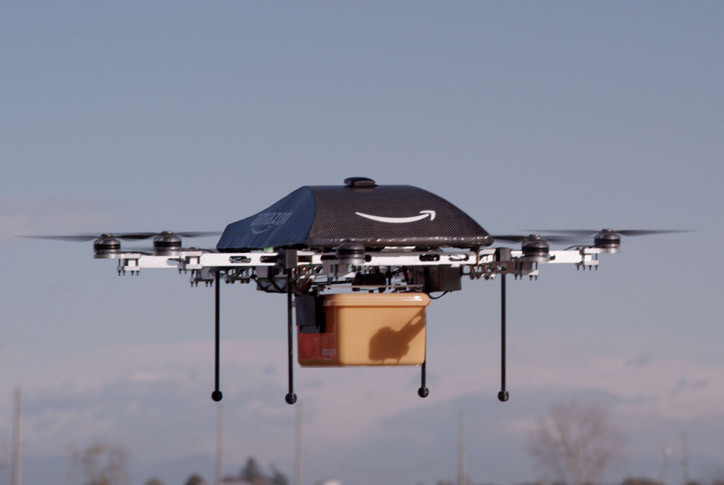
\includegraphics[width=0.28\columnwidth]{./images/drone.jpg}
        }
        \subfloat[]
        {
            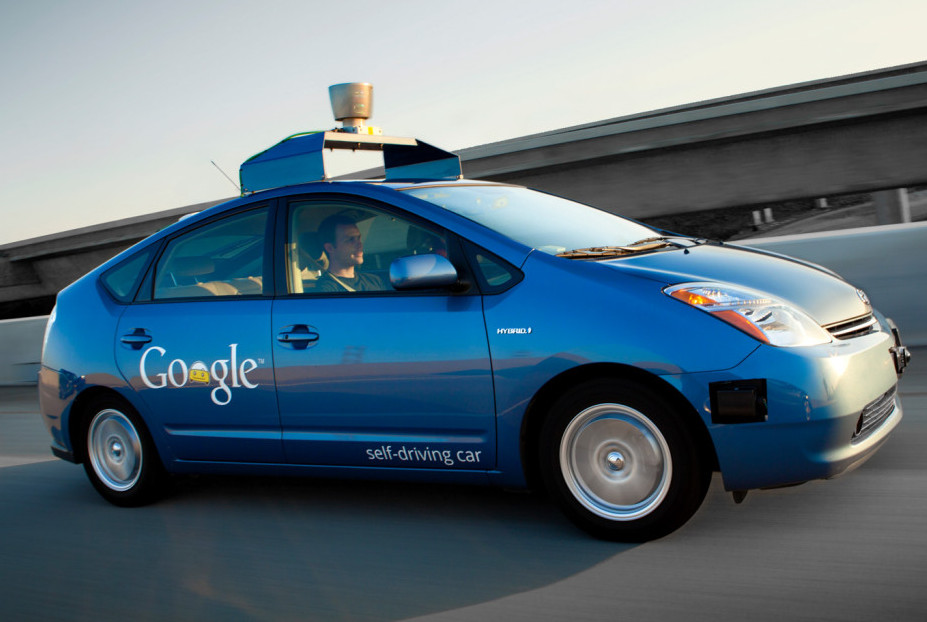
\includegraphics[width=0.28\columnwidth]{./images/google_car.jpg}
        }
        \subfloat[]
        {
            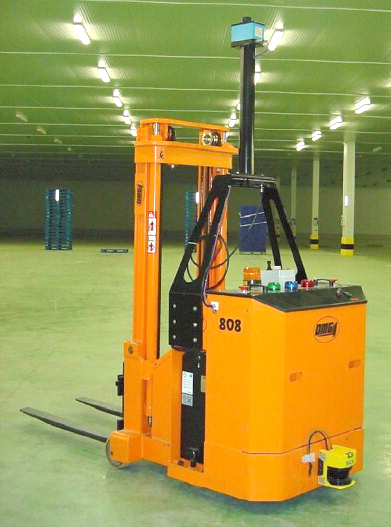
\includegraphics[width=0.14\columnwidth]{./images/industrial_robot.png}
        }\\
        \subfloat[]
        {
            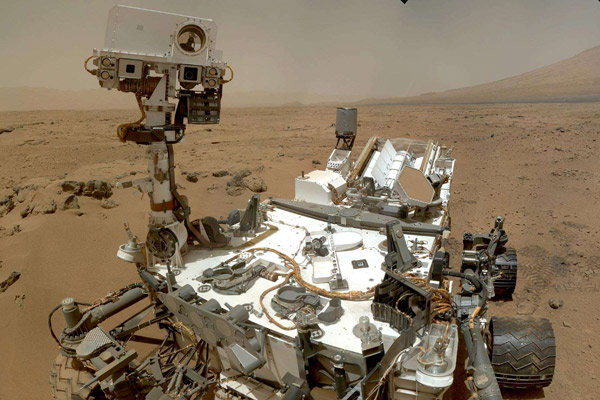
\includegraphics[width=0.34\columnwidth]{./images/curiosity.png}
        }
        \subfloat[]
        {
            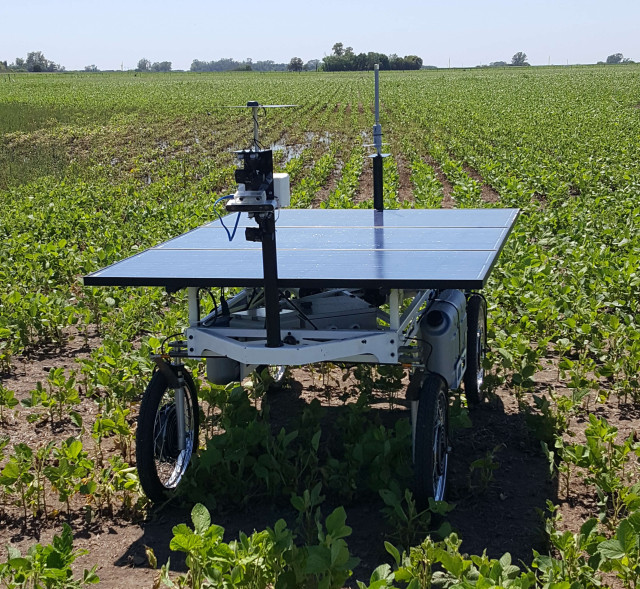
\includegraphics[width=0.25\columnwidth]{./images/weed_removal_robot.jpg}
        }
        \subfloat[]
        {
            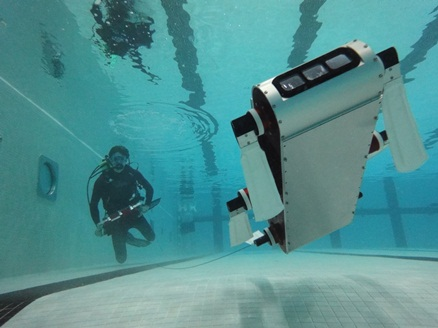
\includegraphics[width=0.31\columnwidth]{./images/aqua.png}
        }
    \end{figure}
\end{frame}

\begin{frame}
    \frametitle{Aplicaciones de la Robótica}

    \begin{columns}[T] % align columns
        \begin{column}{.48\textwidth}
            \begin{itemize}
                \item Vehículos autónomos
                \item Industriales
                \item Cuidado de la Salud
                \item Aeroespacial
                \item Robots de consumo
                \item Respuesta a desastres/catástrofes
                \item Drones (UAV)
            \end{itemize}
        \end{column}%
        \hfill%
        \begin{column}{.48\textwidth}
            \begin{itemize}
                \item Educación
                \item Entretenimiento
                \item Exoesqueletos
                \item Humanoides
                \item Militares
                \item Investigación
                \item Telepresencia
                \item Submarinos
            \end{itemize}
        \end{column}%
    \end{columns}

\TODO{agregar una imagen por cada tipo de robot asi se hacen uan mejor idea}

\end{frame}

\begin{frame}
    \frametitle{Tipos de Robots según locomoción o entorno}

    Brazos robóticos
    Robots con patas
    Robots acuáticos
    Robots Humanoides
    Robots aéreos

\end{frame}


\begin{frame}
    \frametitle{Navegación autónoma}
    \begin{block}{}
        La navegación autónoma puede definirse a grandes rasgos como la capacidad de moverse de forma segura a lo largo de una trayectoria entre un punto de inicio y uno final [1].
    \end{block}
    \vspace{5mm}
    \footnotesize
    \begin{columns}[t]
        \column{0.4\textwidth}
        \hspace{13pt}Pregunta:
        \begin{enumerate}
            \visible<2-7>{ \item[-] ¿Dónde estoy?}
            \visible<4-7>{\item[-] ¿Por dónde estoy yendo?}
            \visible<6-7>{\item[-] ¿Cómo llego hasta allí?}
        \end{enumerate}
        \column{0.6\textwidth}
        Respuesta:
        \begin{enumerate}[$\rightarrow$]
            \visible<3-7>{\item  Cálculo de la posición (Localization)}
            \visible<5-7>{\item  Representación del entorno (Mapping)}
            \visible<7-7>{\item  Planeamiento de trayectoria (Path planning)}
        \end{enumerate}
    \end{columns}
    \only<4>{}
    \vfill
    \begin{tiny}
        [1] J. J. Leonard - et al., ``Mobile robot localization by ...,'' IEEE Transactions on Robotics and Automation, 2002.
    \end{tiny}
\end{frame}

\begin{frame}
    \frametitle{Esquema de control de un robot móvil}
    \begin{figure}[!h]
    	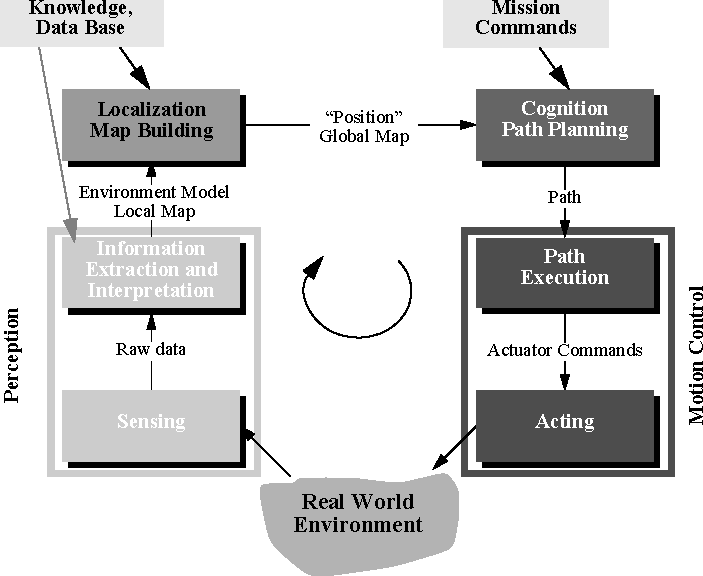
\includegraphics[width=0.6\columnwidth]{mobile_robot_scheme.pdf}
    \end{figure}
\end{frame}

\begin{frame}
    \frametitle{Desafíos de la robótica móvil}

    El entorno, el sistema de locomoción, los sensores y la aplicación determinan los desafíos a resolver.

    \vspace{1em}

    Analizar los problemas que puedan aparecer en ciertas aplicaciones...

    \note{Comentar los problemas actuales del estado del arte. Lor problemas al trabajr con sensores que tienen error, dependiendo el entorno y la aplicación que tiene que hacer el robot hay que resolver diferentes problemas. Dar ejemplos, problemas que hay en el agua, en outdoor con la luz, de noche, blur, comentar problemas con las camaras}
\end{frame}

\begin{frame}
    \frametitle{Impacto de la robótica}

    Filosofemos...
    Revolución industrial.

    \note{Filosofía de la robótica}
\end{frame}
